\documentclass[a4 paper]{article}
% Set target color model to RGB
\usepackage[inner=2.0cm,outer=2.0cm,top=2.5cm,bottom=2.5cm]{geometry}
\usepackage{setspace}
\usepackage[rgb]{xcolor}
\usepackage{verbatim}
\usepackage{subcaption}
\usepackage{amsgen,amsmath,amstext,amsbsy,amsopn,tikz,amssymb,tkz-linknodes}
\usepackage{fancyhdr}
\usepackage[obeyspaces,spaces]{url}
\usepackage[colorlinks=true, urlcolor=blue,  linkcolor=blue, citecolor=blue]{hyperref}
\usepackage[colorinlistoftodos]{todonotes}
\usepackage{rotating}
%\usetikzlibrary{through,backgrounds}
\hypersetup{
pdfauthor={Ashudeep Singh},
pdftitle={Assignment 4},
pdfkeywords={Tikz,latex,bootstrap,uncertaintes},
pdfcreator={PDFLaTeX},
pdfproducer={PDFLaTeX},
}
%\usetikzlibrary{shadows}
% \usepackage[francais]{babel}
\usepackage{hyperref}
\usepackage{booktabs}
\usepackage{graphicx}
\usepackage[section]{placeins}
\newcommand*{\figuretitle}[1]{%
    {\centering%   <--------  will only affect the title because of the grouping (by the
    \textbf{#1}%              braces before \centering and behind \medskip). If you remove
    \par\medskip}%            these braces the whole body of a {figure} env will be centered.
}
\newcommand{\ra}[1]{\renewcommand{\arraystretch}{#1}}

\newtheorem{thm}{Theorem}[section]
\newtheorem{prop}[thm]{Proposition}
\newtheorem{lem}[thm]{Lemma}
\newtheorem{cor}[thm]{Corollary}
\newtheorem{defn}[thm]{Definition}
\newtheorem{rem}[thm]{Remark}
\numberwithin{equation}{section}

\newcommand{\homework}[6]{
   \pagestyle{myheadings}
   \thispagestyle{plain}
   \newpage
   \setcounter{page}{1}
   \noindent
   \begin{center}
   \framebox{
      \vbox{\vspace{2mm}
    \hbox to 6.28in { {\bf COMP 3005:~Database Management Systems \hfill {\small (#2)}} }
       \vspace{6mm}
       \hbox to 6.28in { {\Large \hfill #1  \hfill} }
       \vspace{6mm}
       \hbox to 6.28in { {\it Instructor: {\rm #3} \hfill Name: {\rm #5}, ID: {\rm #6}} }
       %\hbox to 6.28in { {\it TA: #4  \hfill #6}}
      \vspace{2mm}}
   }
   \end{center}
   \markboth{#5 -- #1}{#5 -- #1}
   \vspace*{4mm}
}

\newcommand{\problem}[2]{~\\\fbox{\textbf{Q #1}}\hfill (#2 points)\newline\newline}
\newcommand{\subproblem}[1]{~\newline\textbf{(#1)}}
\newcommand{\D}{\mathcal{D}}
\newcommand{\Hy}{\mathcal{H}}
\newcommand{\VS}{\textrm{VS}}
\newcommand{\solution}{~\newline\textbf{\textit{(Solution)}} }

\newcommand{\bbF}{\mathbb{F}}
\newcommand{\bbX}{\mathbb{X}}
\newcommand{\bI}{\mathbf{I}}
\newcommand{\bX}{\mathbf{X}}
\newcommand{\bY}{\mathbf{Y}}
\newcommand{\bepsilon}{\boldsymbol{\epsilon}}
\newcommand{\balpha}{\boldsymbol{\alpha}}
\newcommand{\bbeta}{\boldsymbol{\beta}}
\newcommand{\0}{\mathbf{0}}


\begin{document}
\homework{Look Inna Book}{Due: Friday Apr. 3, 2020 (11:59 PM)}{Ahmed El-Roby}{}{Devon Hope}{101038344}

\tableofcontents
\newpage
\section{Conceptual Design}
\qquad This section explains and demonstrates how the database uses the ER-Diagram to store and hold all neccessary information given in the project summary. 
\subsection{ER-Diagram}
{\centering 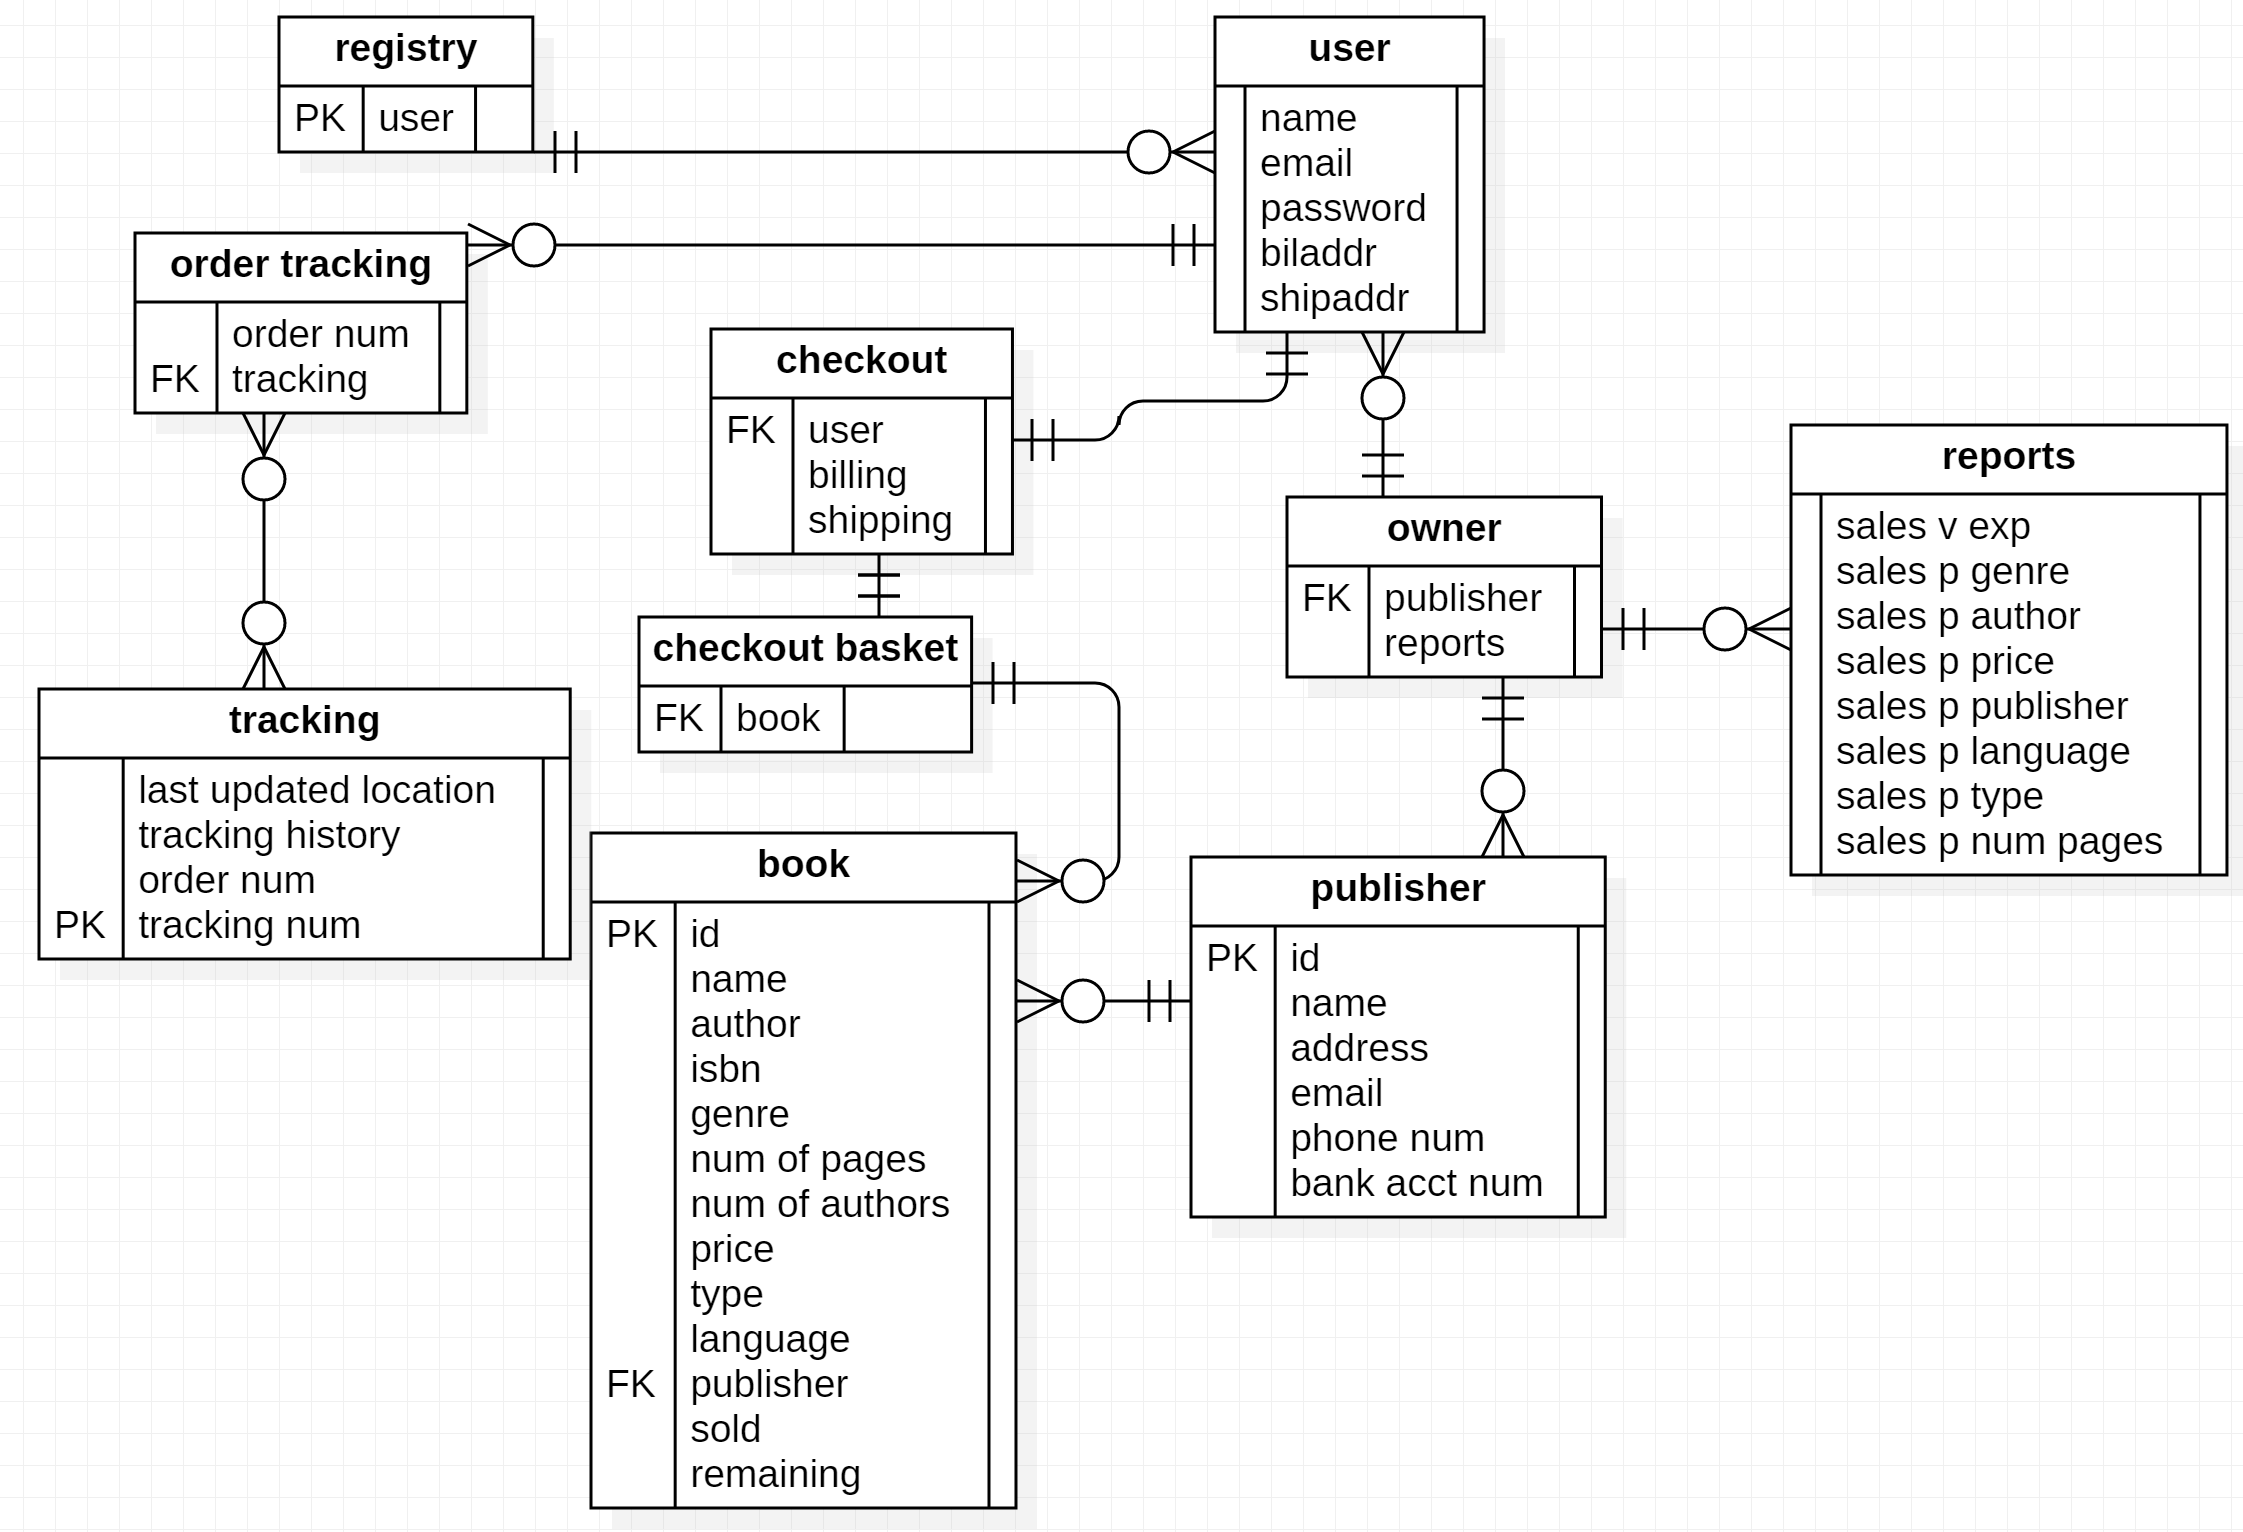
\includegraphics[width=\textwidth/1]{ER_D.png}}
\subsection{Explanation}
\qquad This diagram contains all of the necessary entities to store all necessary information created by and used by the user in the program during runtime. All user information is stored in the user entity when they are signed into the program, this way everything they need is easily accessible. All of the users cart and checkout information is stored in the entities checkout and checkout basket, checkout stores the user id, records their shipping and billing addresses, and checkout basket stores all of the books in the users cart, the book entity is a foreign key for the book entity. When the user goes to checkout their cart, and is successful, all tracking information for their order is stored in the order tracking entity and the final tracking information from the third party shipping company is given and stored in the tracking entity. The tracking entity is a foreign key for the order tracking entity. The publisher entity holds all information needed by the user and the owner of the store on each publisher, the user only needs a name whereas the owner can see all other information required. The owner entity holds all of the relevant information for the owner, such as the a foreign key for the publisher entity id. The reports entity holds all of the reports created by the program. 
\section{Reduction to Relation Schemas}
{\centering 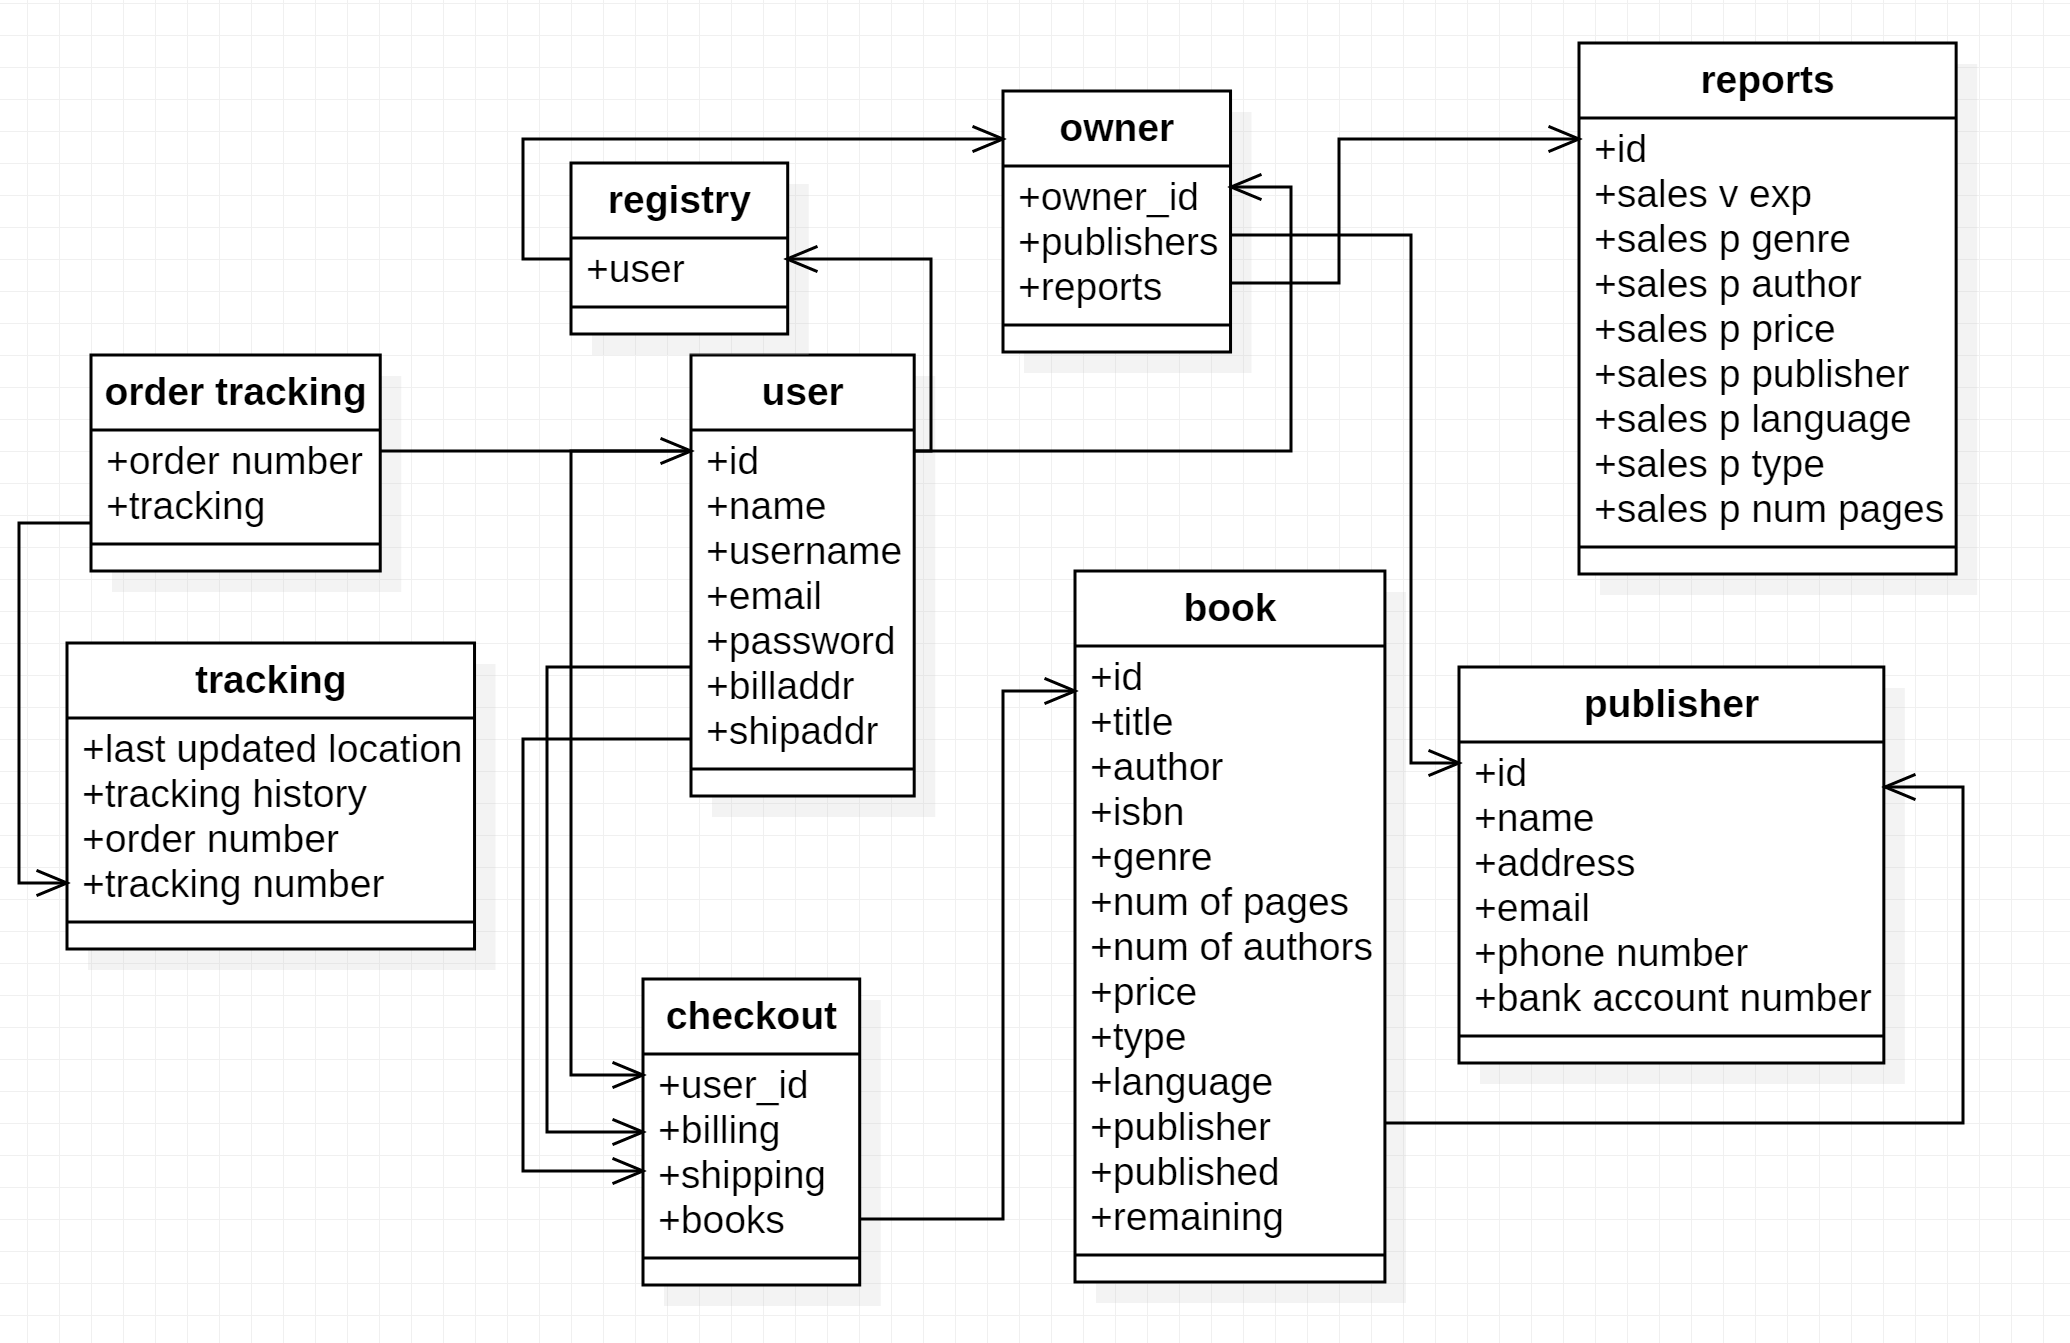
\includegraphics[width=\textwidth/1]{RS_D.png}}
\section{Normalization of Relation Schemas}
\subsection{Normalization}
{\centering 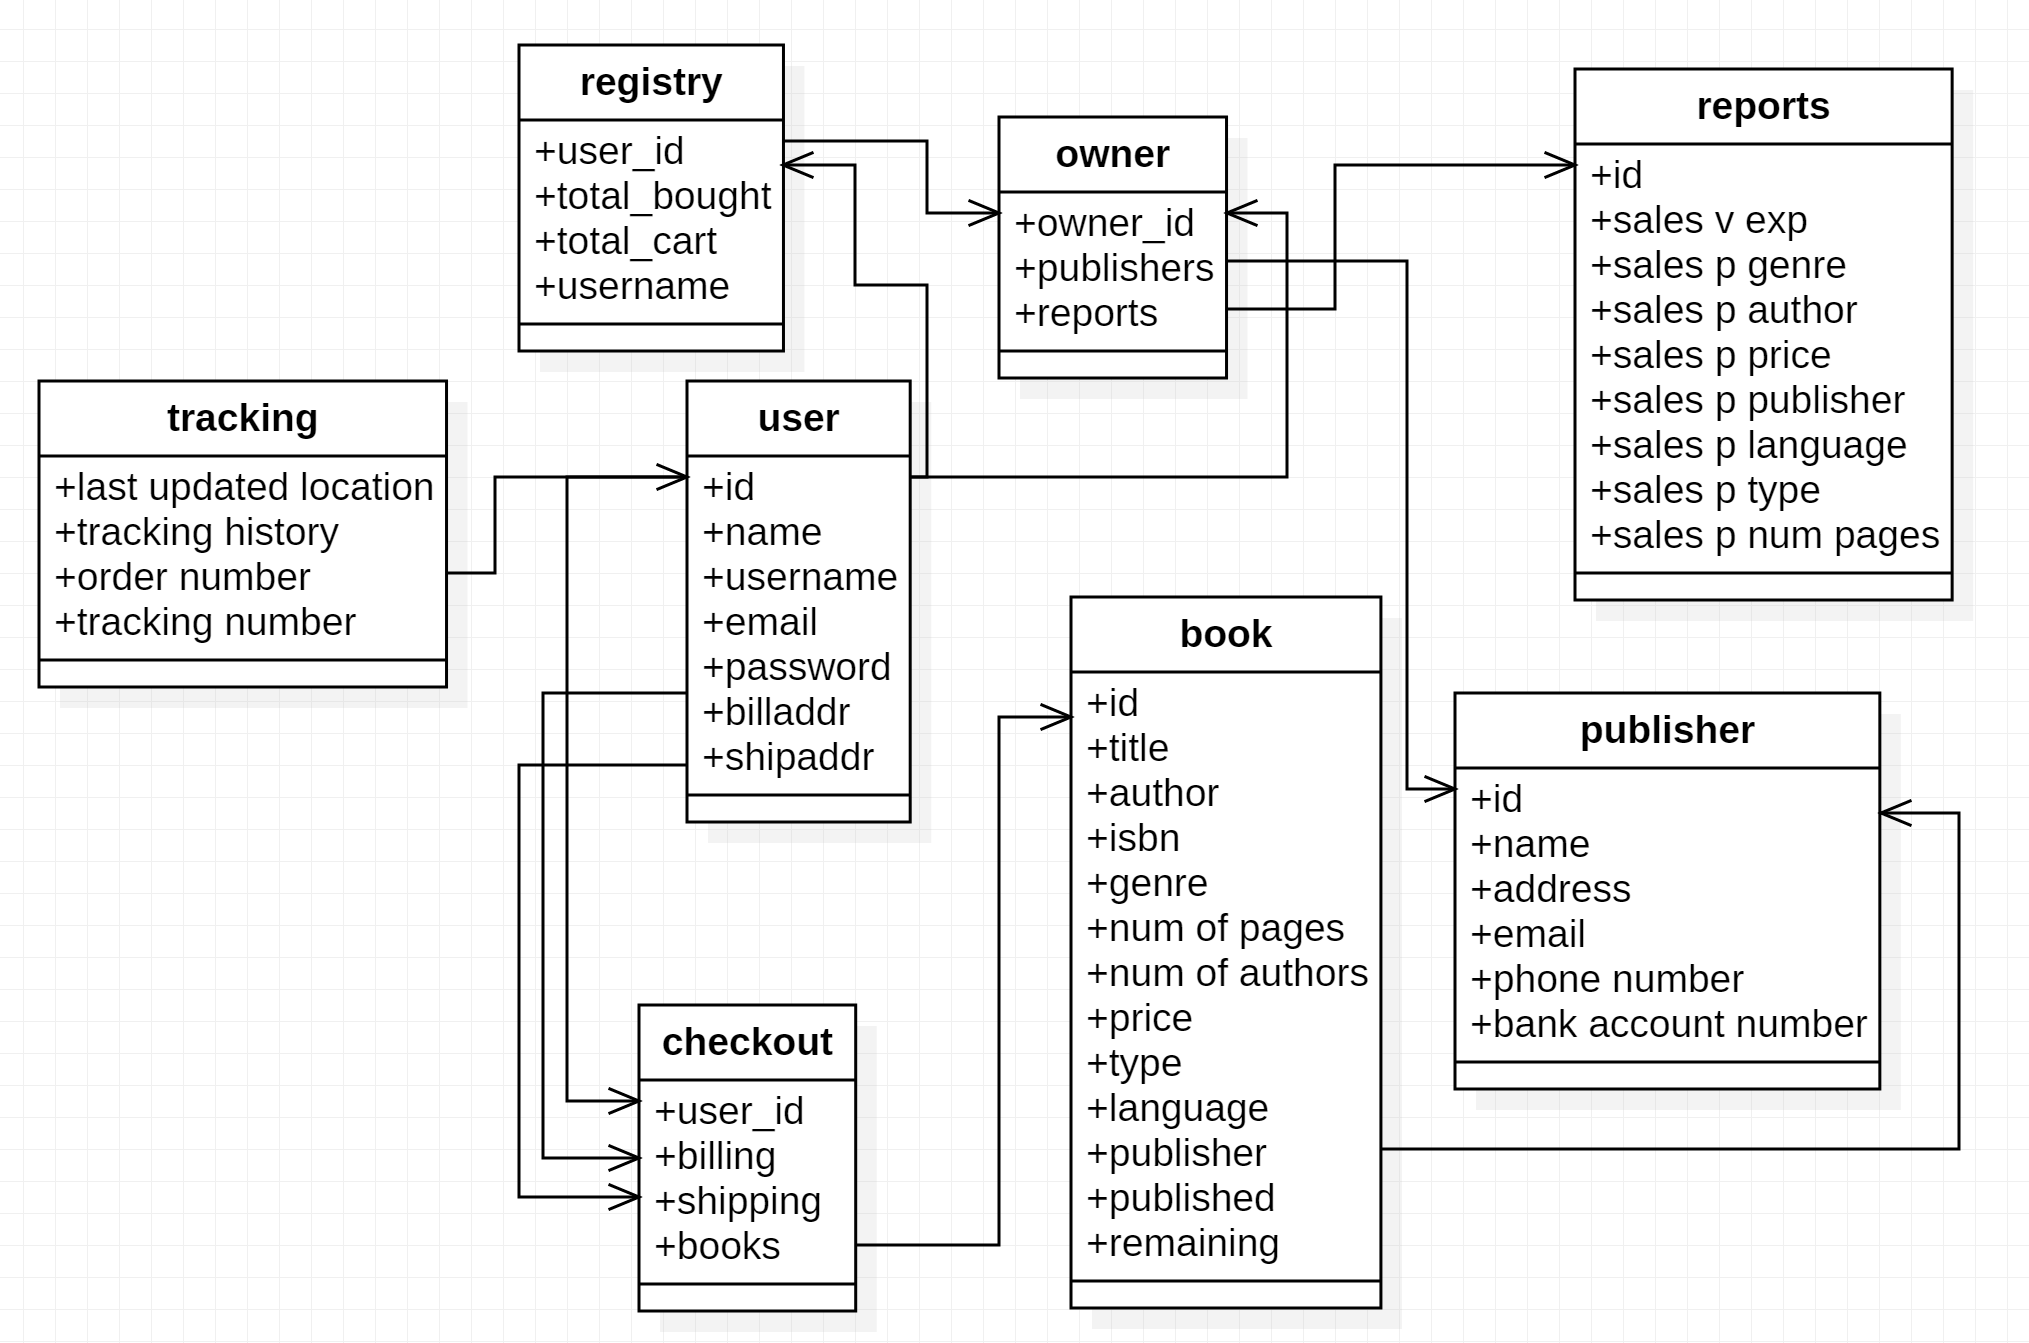
\includegraphics[width=\textwidth/1]{NRS_D.png}}
\subsection{Explanation}
\qquad Every schema passes the 1NF test but the registry schema, this registry holds a user id, that is a unique string that contains the id of the user, a total of the books they have bought and the books in their cart. These three attributes in one string are usually well defined for each user and are not easily replicable. This could or could not pass the 1NF test, I personally would pass it, but if this was to be released globally, I would decompose it and reconstruct it into four or five defining attributes including the user\_id, user\_username, total\_books, total\_cart and or user\_email. As for order tracking, I believe it passes the first test, 1NF, and the second, 2NF, as for the third one, it does have transitive functional properties, specifically the attribute tracking. To allow for all three tests, tracking could absorb order tracking, as they have similar attributes, and one of them is transitive, this was initially designed to create a layer of security, but ultimately does not work in a functioning practice. 
\section{Database Schema Diagram}
{\centering 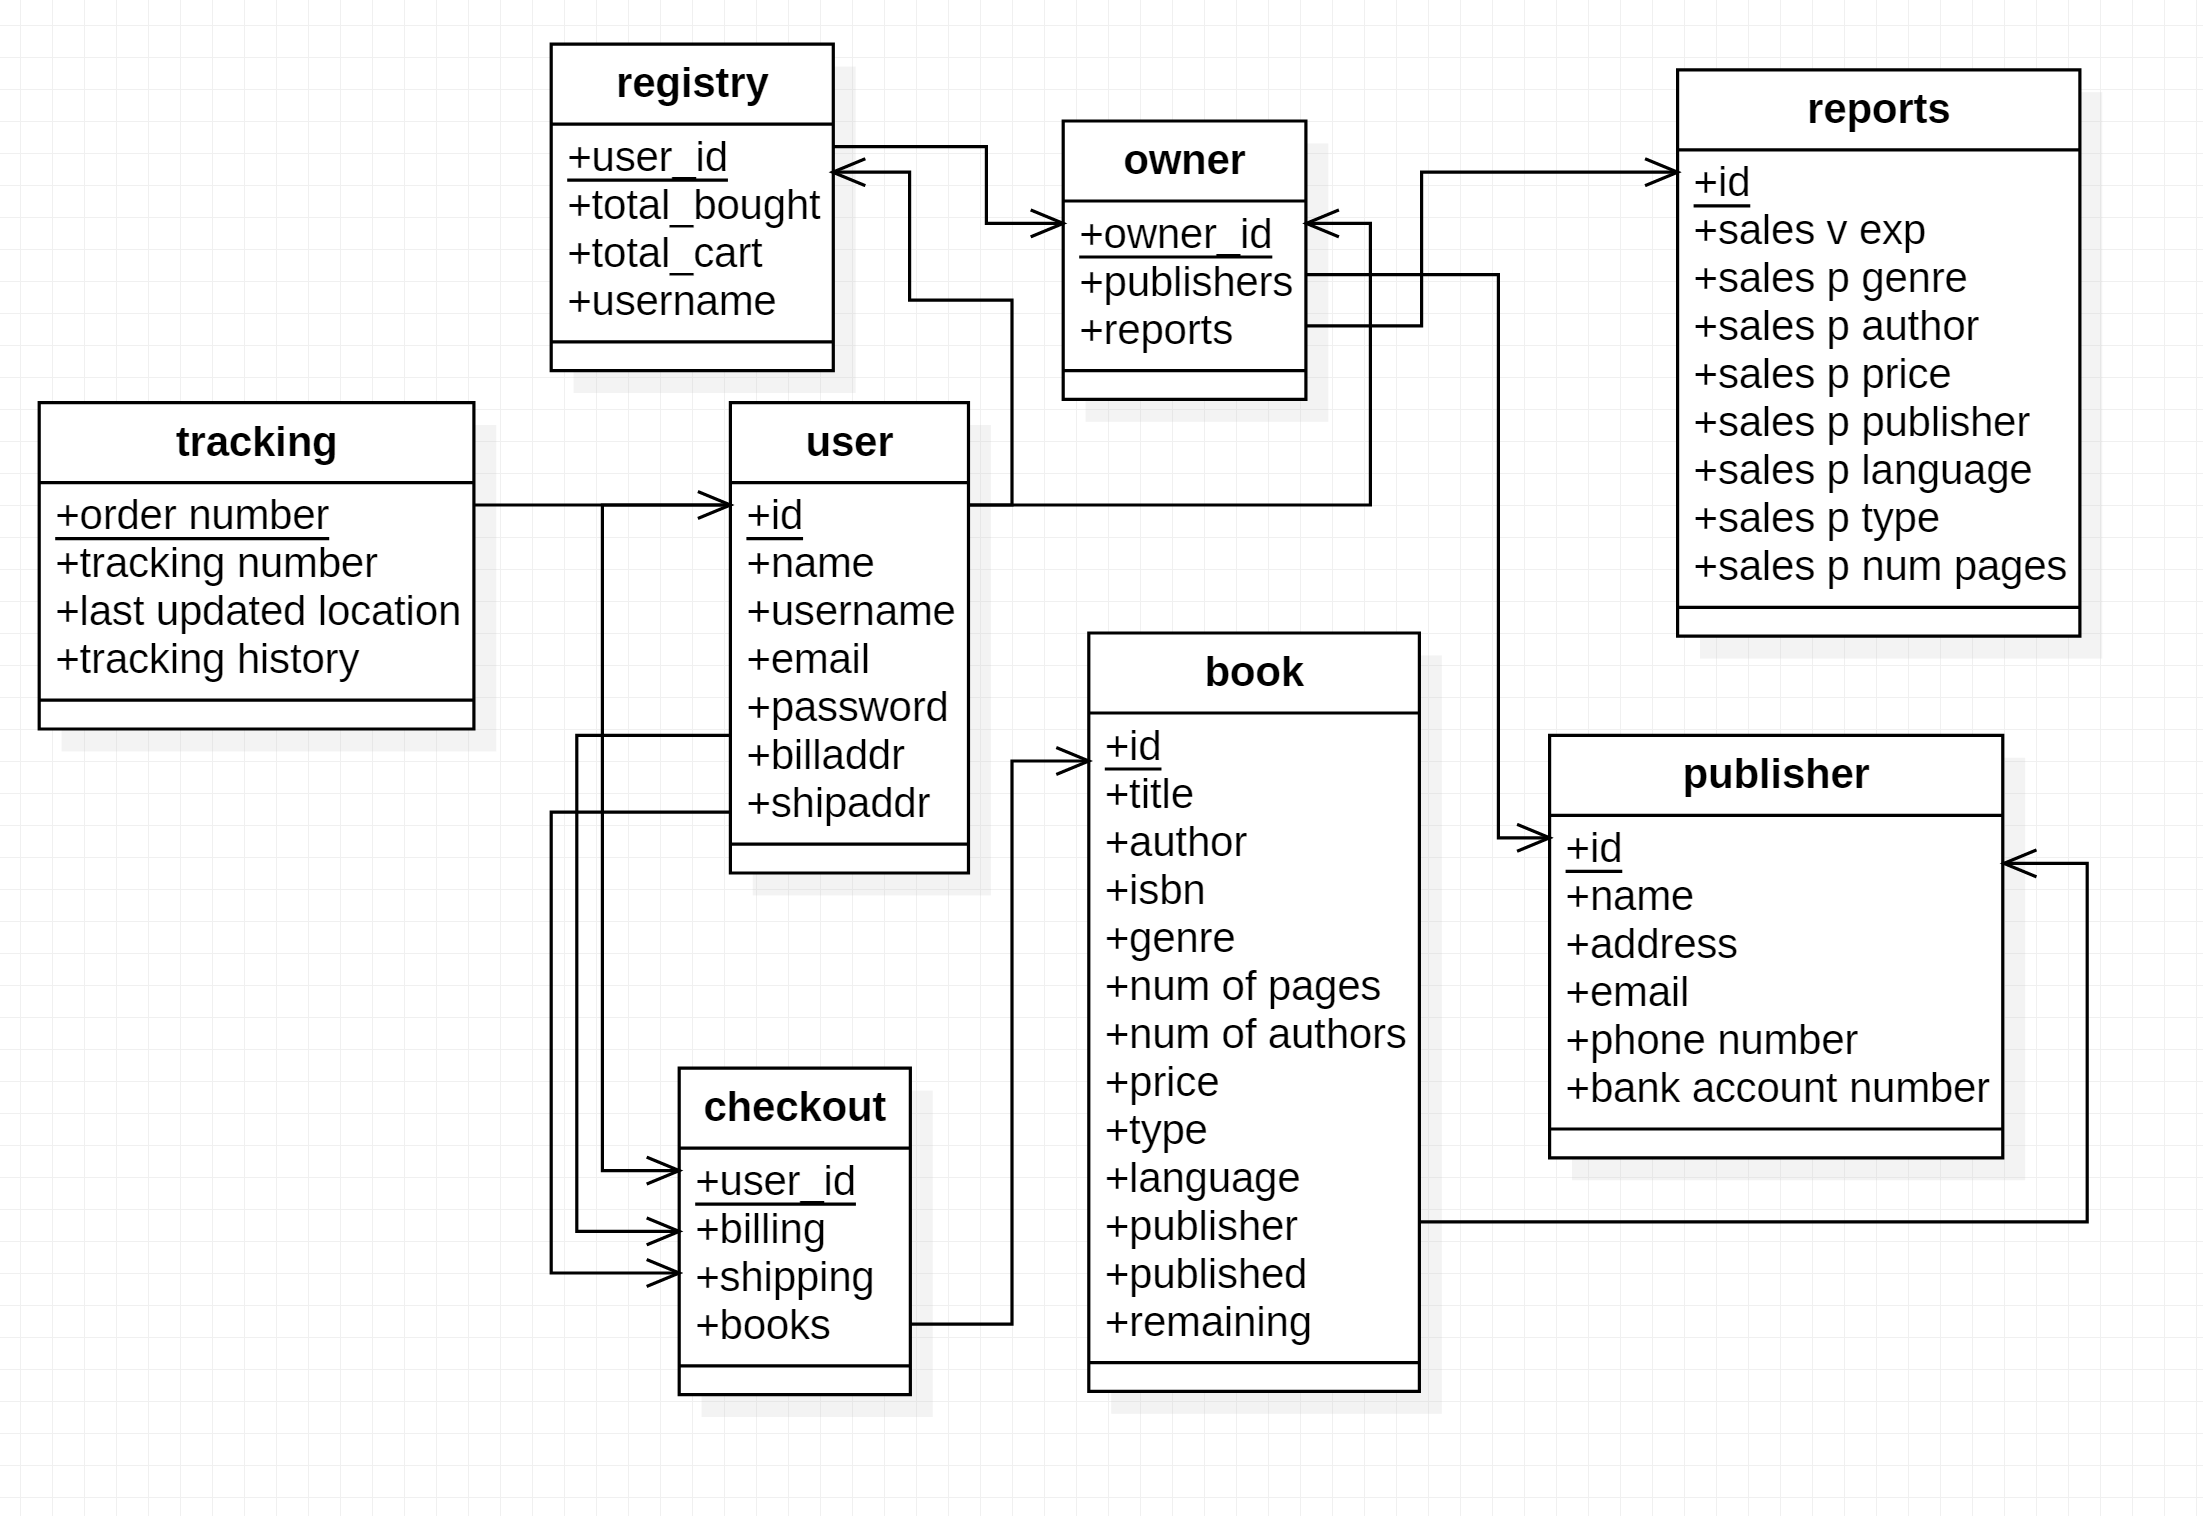
\includegraphics[width=\textwidth/1]{Schema_D.png}}
\section{Implementation}
\subsection{Overview}
\qquad I tried to complete the user and owner front end with a node.js web client but I couldn't before the due date, instead I implemented most of the user features, excluding the checkout and tracking in a command line version. I have pushed all versions of my project, whether complete or incomplete, to my github attached below. The version that works the best is under the directory `lib\_app', it uses python to query and connect to the postgresql and as an interface with the user. 
\subsection{Scenarios}
\subsubsection{lib\_app}
These are stills of basic scenarios that have been imeplemented so far. Hopefully most if not all of the implementation is done before the due date, although this is a large program. The program is simple, its menu based, you select your options  and give answers to questions like what book you want or which option number to choose. These basic scenarios contain stills of the main menu, signing in, browsing the books, displaying more information on a specific book, searching for a specific book, adding books to your cart and displaying you cart\\\\
\begin{figure}
\centering 
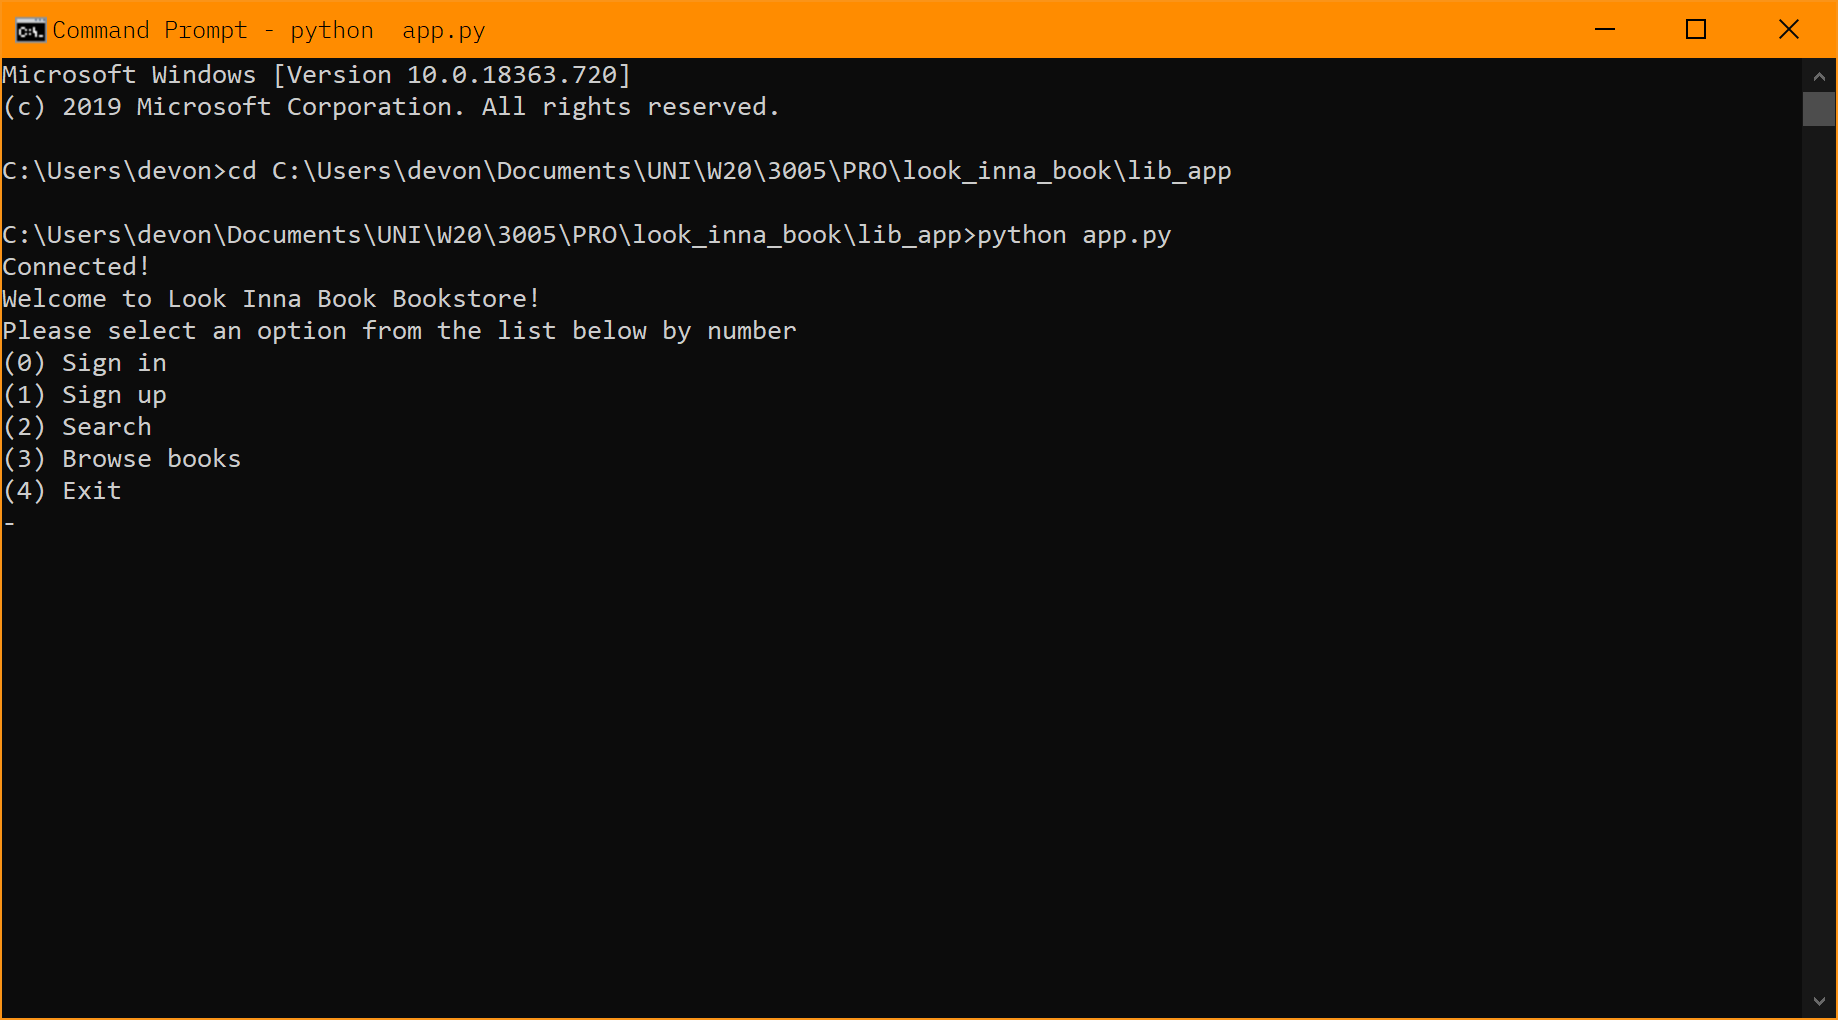
\includegraphics[width=\textwidth/1]{scenarios_cmd/Main_menu.png} 
\caption{Main Menu}
\end{figure}
\begin{figure}
\centering 
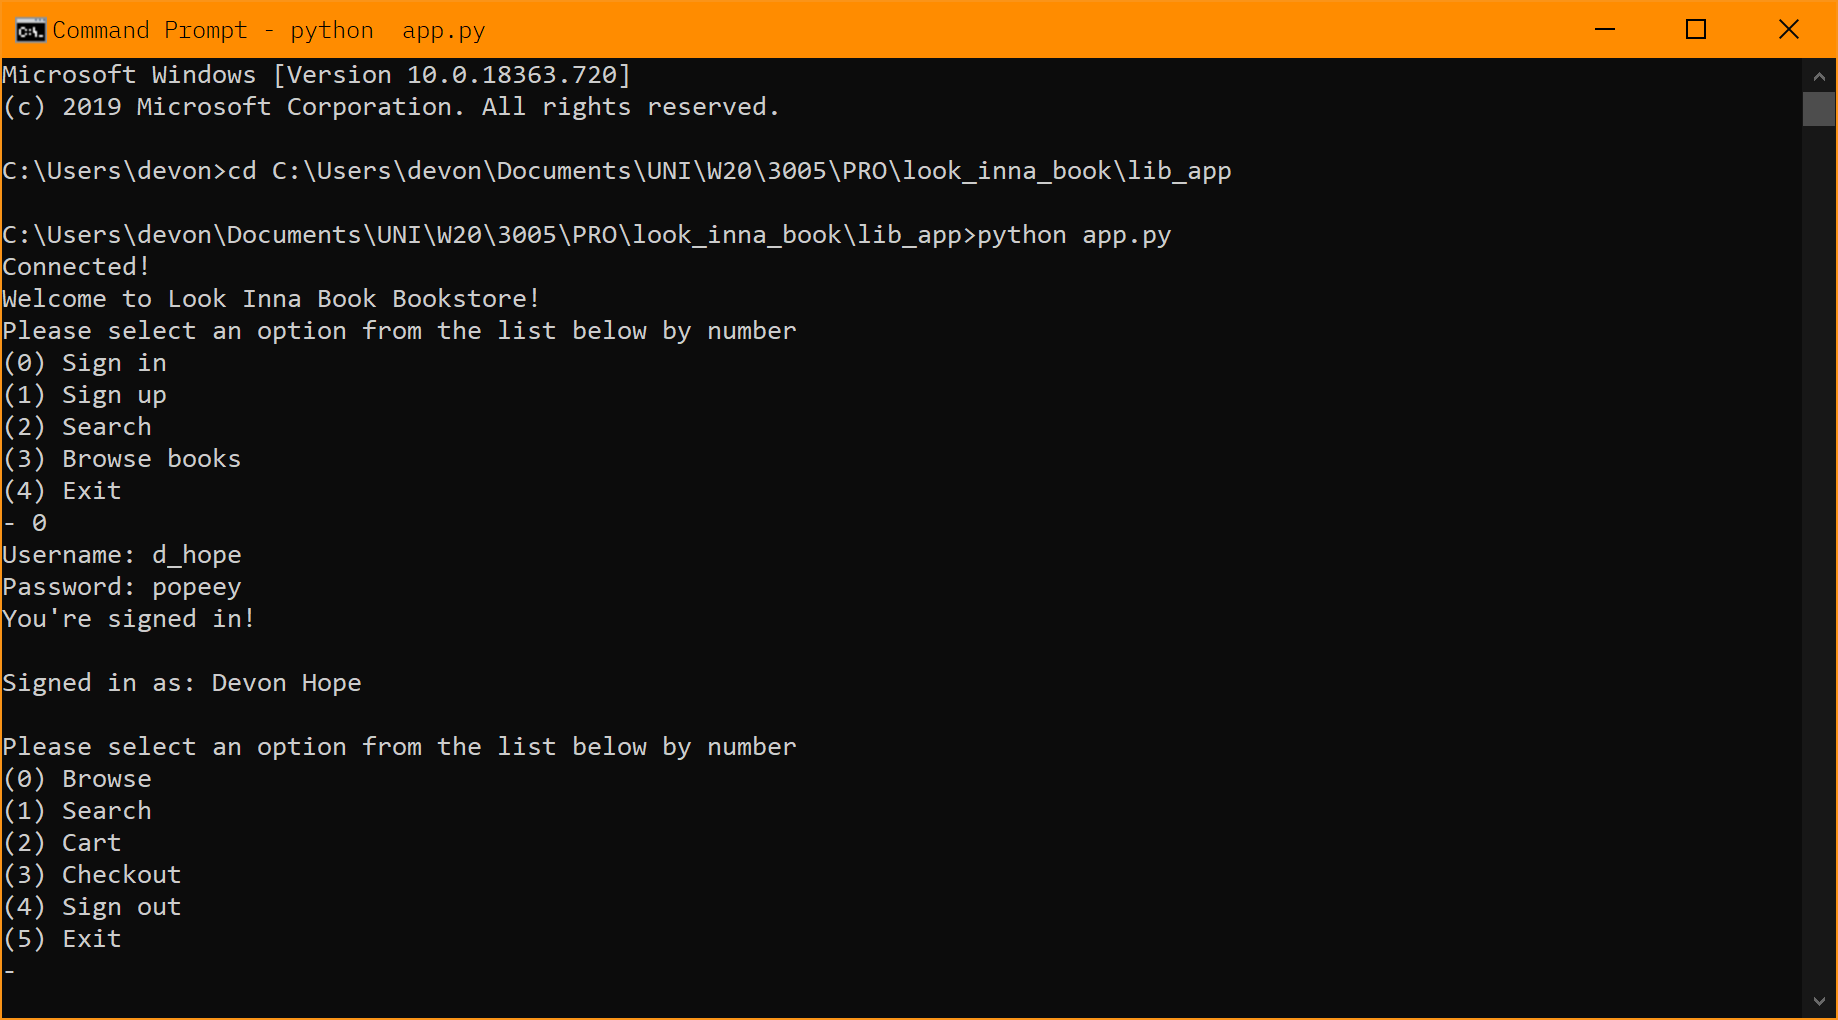
\includegraphics[width=\textwidth/1]{scenarios_cmd/signed_in_menu.png}
\caption{Signed in Menu}
\end{figure}
\begin{figure}
\centering 
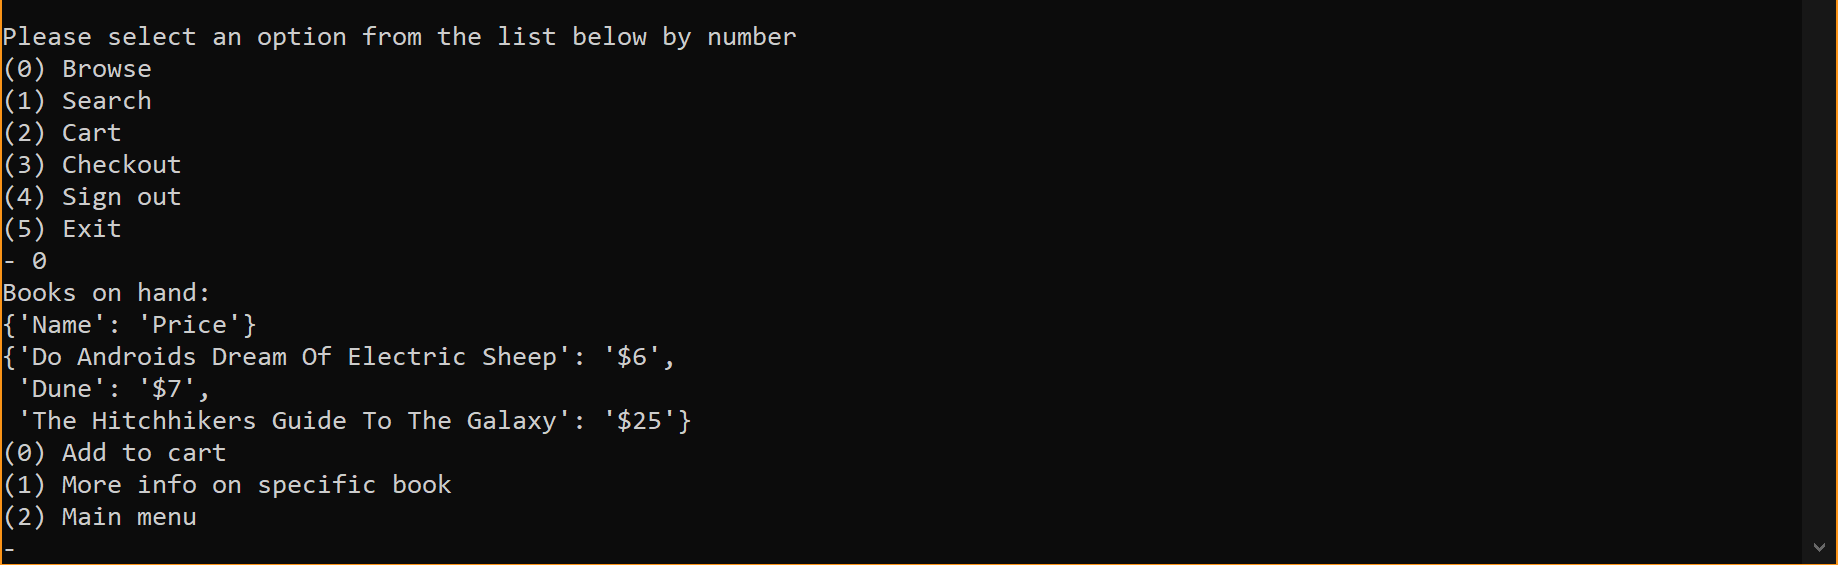
\includegraphics[width=\textwidth/1]{scenarios_cmd/browse_menu.png}
\caption{Browse the books}
\end{figure}
\begin{figure}
\centering 
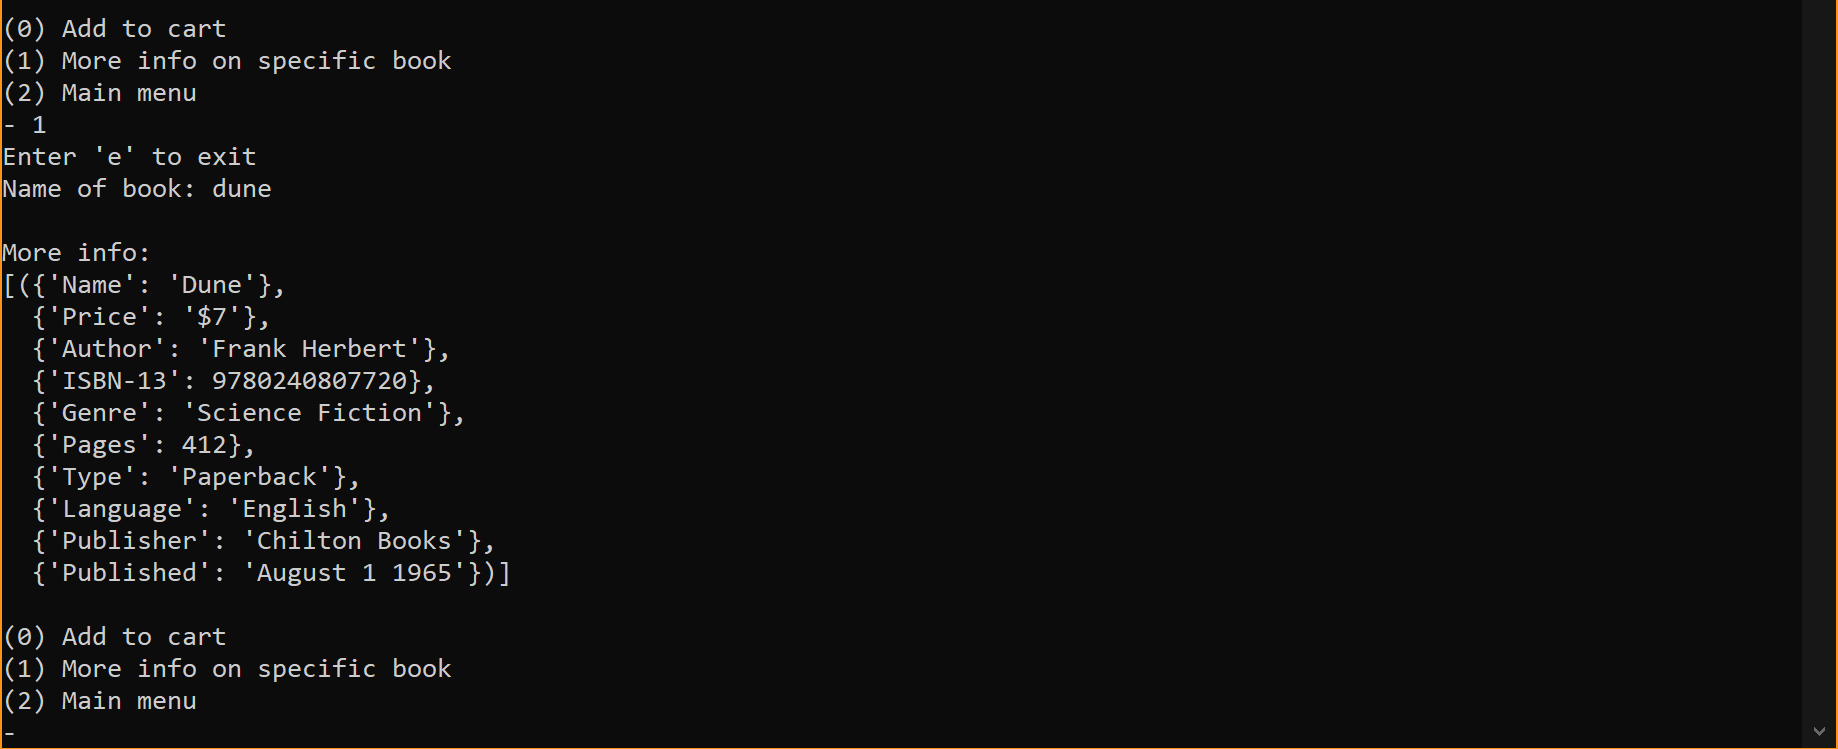
\includegraphics[width=\textwidth/1]{scenarios_cmd/more_info.png}
\caption{More information on a book}
\end{figure}
\begin{figure}
\centering 
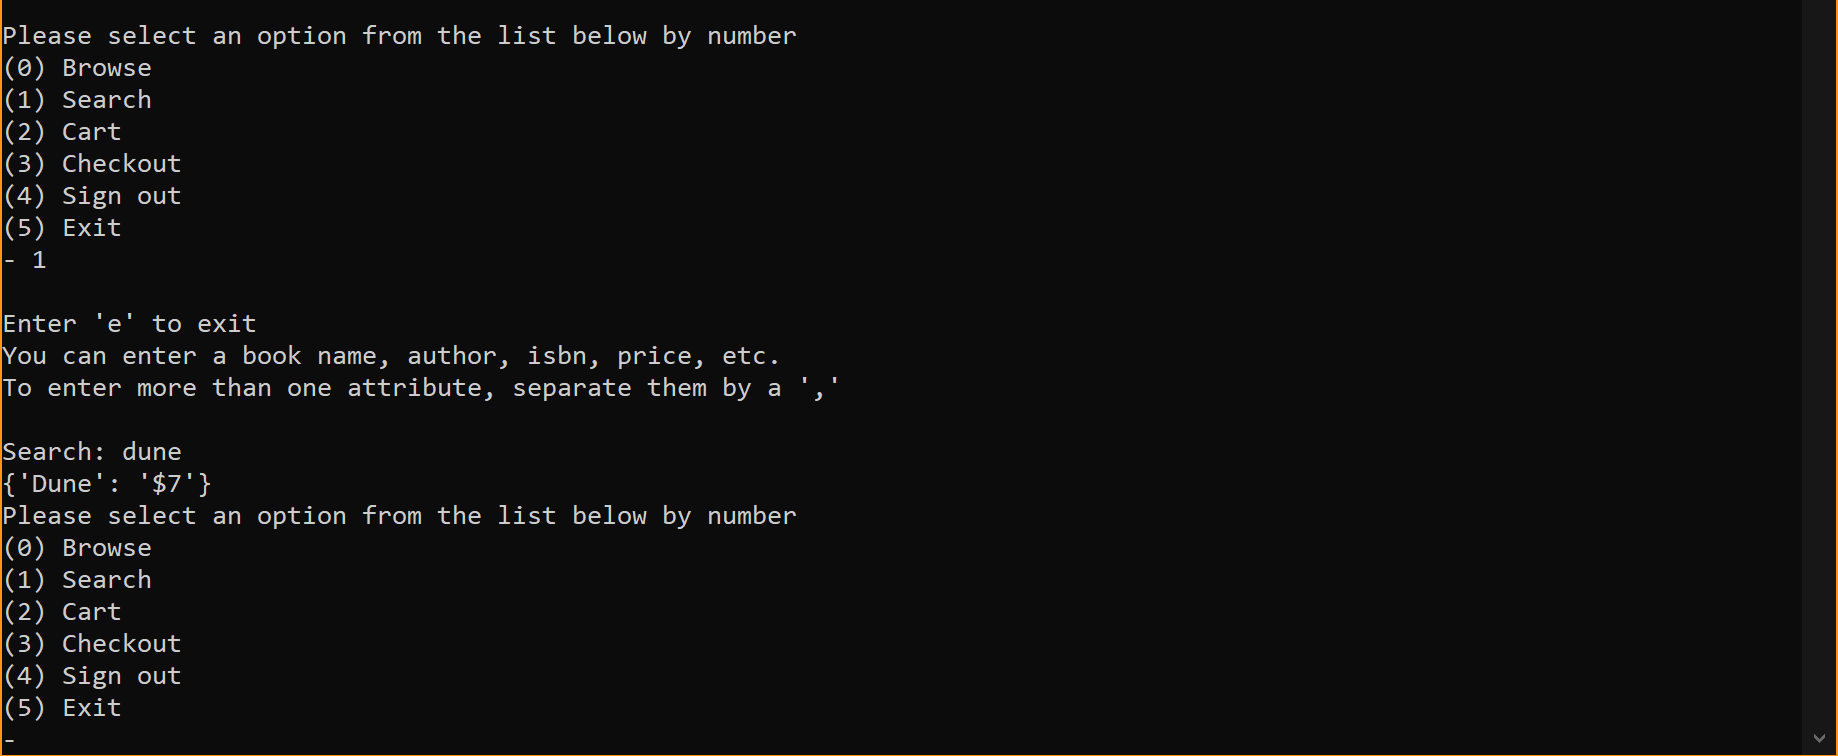
\includegraphics[width=\textwidth/1]{scenarios_cmd/search.png}
\caption{Searching for a specific book}
\end{figure}
\begin{figure}
\centering 
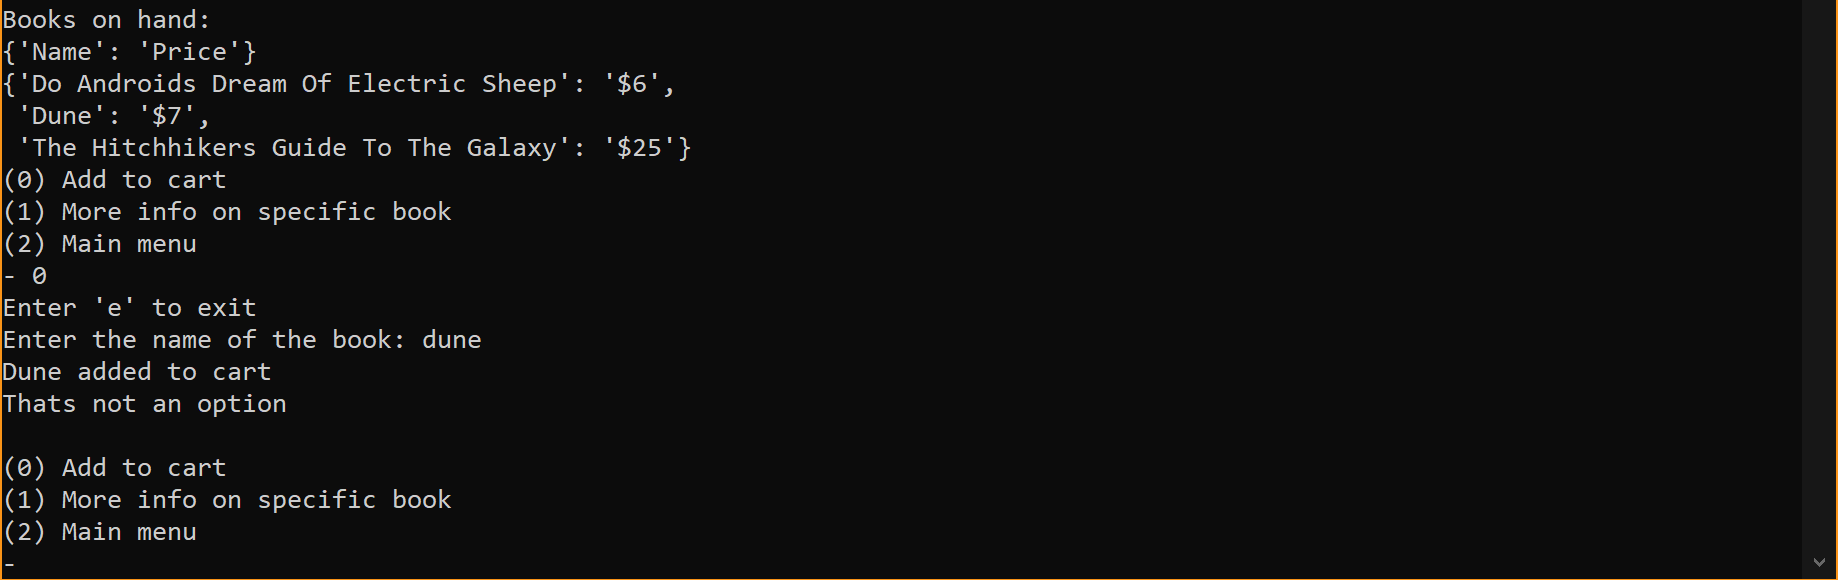
\includegraphics[width=\textwidth/1]{scenarios_cmd/adding_to_cart.png}
\caption{Adding books to your cart}
\end{figure}
\begin{figure}
\centering 
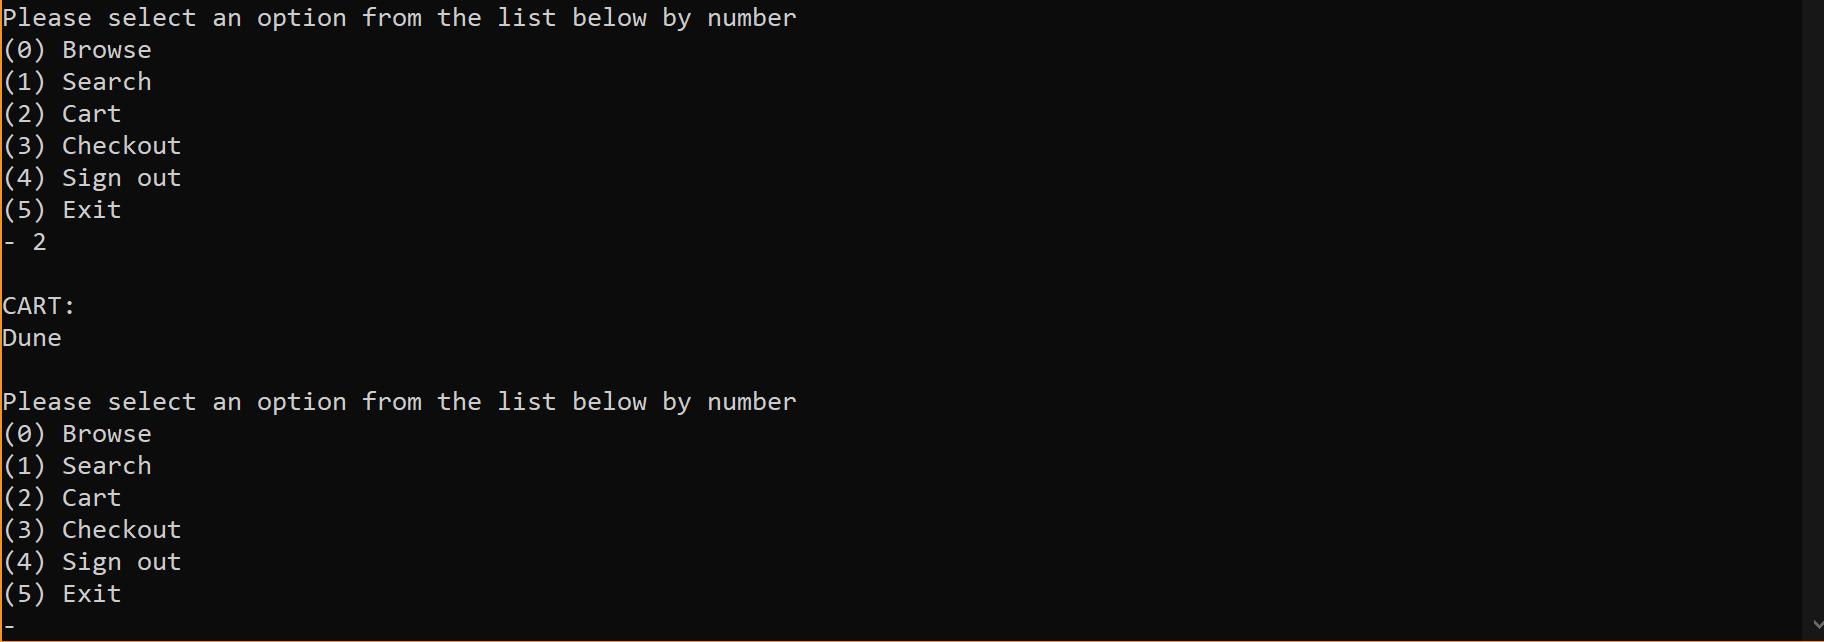
\includegraphics[width=\textwidth/1]{scenarios_cmd/cart.png}
\caption{Displaying your cart}
\end{figure}
\section{Github Repostiory}
\href{https://github.com/WalterMitty2112/Online-Bookstore-Webapp}{Git Repo (Look Inna Book: Online Bookstore)}
\section{Instructions for Submission}
\begin{enumerate}
\item Ensure that PostgreSQL is running on your machine, if not then install and run 
\item Create a database called Bookstore under a postgrsql 12 server
\item Open a terminal or cmd for windows
\item Navigate to \path{C:\Program Files\PostgreSQL\12\bin} or the bin folder of the latest version of your postgresql folder installed on your machine
\item Open the folder \path{\lib_app\pgdb} under the \path{lib_app} inside the project folder and copy the directory to the file \path{lib_app\pgdb\latest_db_back.sql} file
\item Change the command below to add your username and directory path to the file \path{latest_db_backsql}: \\
\path{psql -U <username> Bookstore < ..\look_inna_book\lib_app\pgdb\latest_db_back.sql}
\item Enter the password for your postgresql server\\\\
NOTE: The command above, updates the currently running postgresql server with my database structure and data
\end{enumerate}
\subsection{lib\_app}
\begin{enumerate}
\item Esnure python3 or later is installed on your machine by opening a terminal and typing: \path{python --version}
\item Open the file \path{cred_pgsql.py}
\item Change the variables PGUSER and PGPASSWORD to your postgrsql username and password for the server
\item To run the program, navigate to the \path{lib_app} folder use the command: \path{python app.py}
\end{enumerate}

\end{document}